%\section{Introduction}
\label{sec:introduction}

Reading text in images is still an open problem in computer vision and image understanding research fields. This problem has attracted a lot of attention to these communities due to a large number of modern applications that can potentially benefit from this knowledge, such as self-driving vehicles~\cite{Yan2018TITS,Zhu2018TITS}, robot navigation, scene understanding~\cite{Wang2018IJCV}, assistive technologies~\cite{Yi2014TM}, among others. In addition, the ubiquity of mobile and wearable devices led the text detection and recognition problems to a high-order complexity in terms of efficiency and effectiveness, as both are expected to be performed in real-time in several practical usage scenarios. Thereby, the conception of methods for understanding texts in images effectively and at low computation costs is of paramount importance.

Several methods have been recently proposed in the literature towards localizing textual information in scene images. In general, the text reading problem comprises two distinct tasks: localization and recognition. The former seeks to localize delimited candidate regions that contain textual information, while the second is responsible for transcribing the text inside the candidate regions found during the localization task.
In both tasks, the inherent variability of a text (e.g., size, color, font style, background clutter, and perspective distortions), as illustrated in Fig.~\ref{fig:problematic_images},
makes the text reading a very challenging problem.

\begin{figure}[!ht]
    \centering
    \includegraphics[width=0.40\textwidth]{dataset_samples/icdar13/img_27.jpg}
    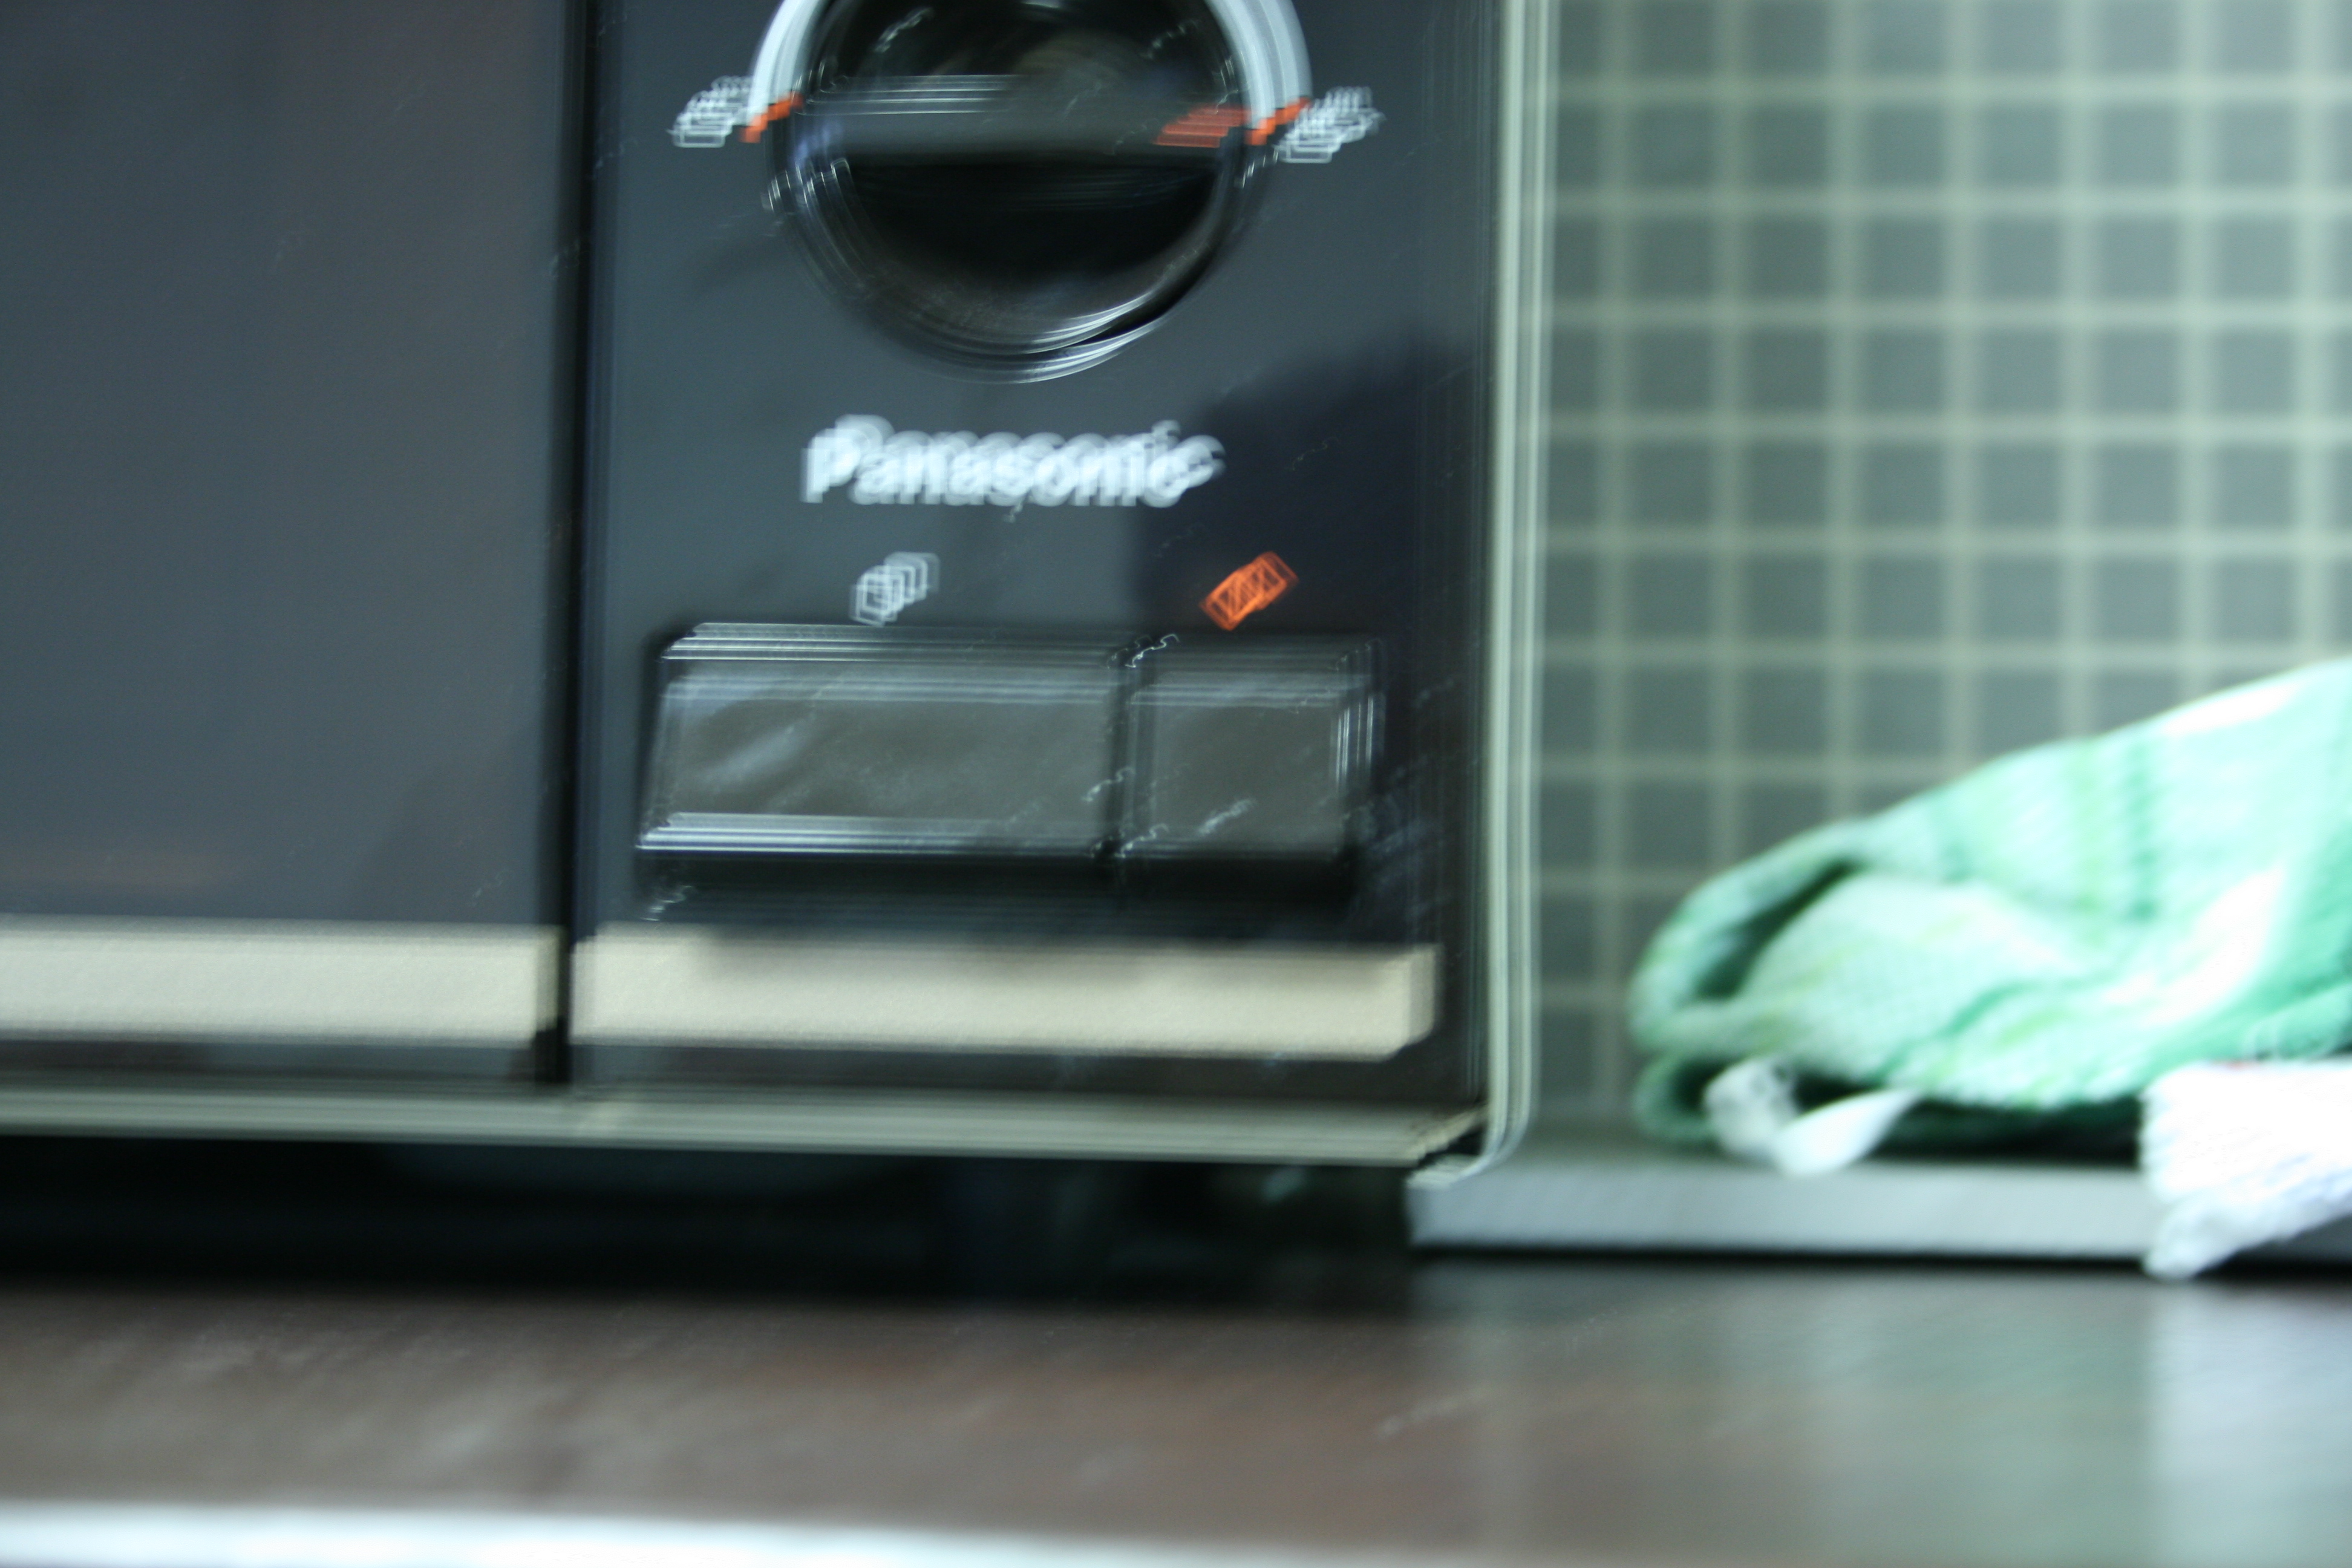
\includegraphics[width=0.40\textwidth]{dataset_samples/icdar13/img_169.jpg}
    
    \vspace{1.5mm}
    
    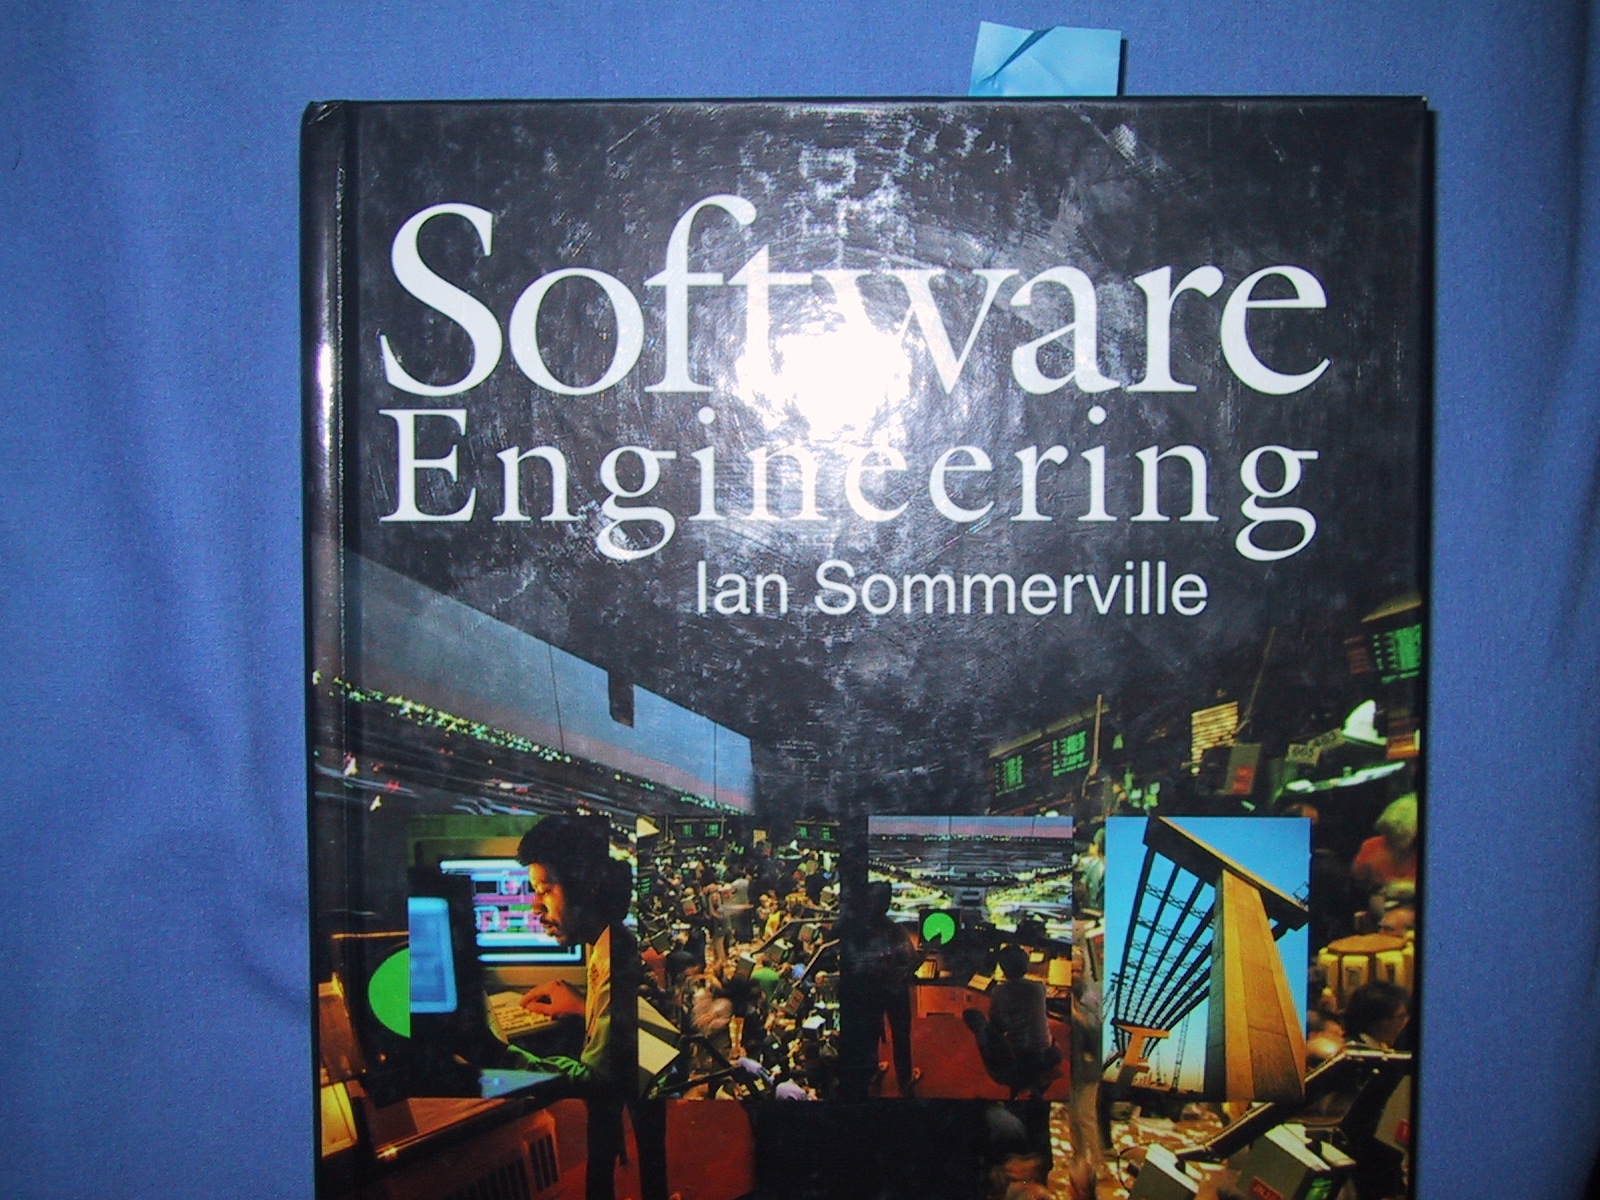
\includegraphics[width=0.40\textwidth]{dataset_samples/icdar13/img_37.jpg}
    
\includegraphics[width=0.40\textwidth]{dataset_samples/icdar13/img_40.jpg}
    
    \vspace{1.5mm}
    
    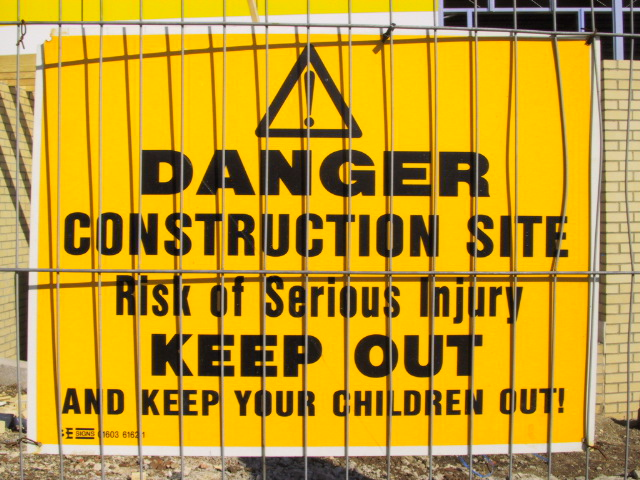
\includegraphics[width=0.40\textwidth]{dataset_samples/icdar13/img_107.jpg}
    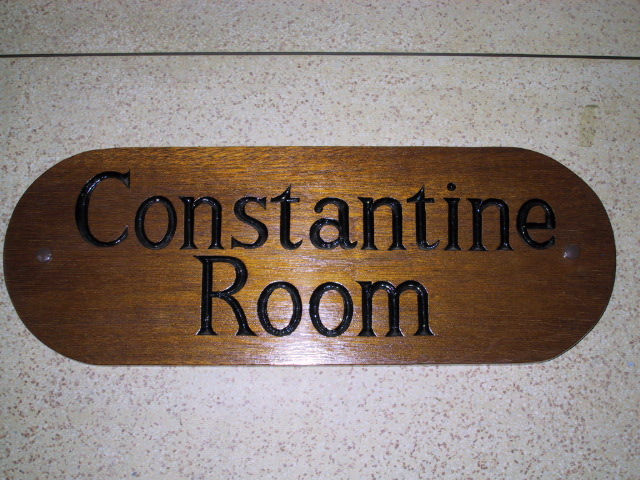
\includegraphics[width=0.40\textwidth]{dataset_samples/icdar13/img_207.jpg}
    \caption{Examples of scene text images with challenging visual properties.}
    \label{fig:problematic_images}
\end{figure}

%
%\begin{figure}[!t]
%	\centering
%	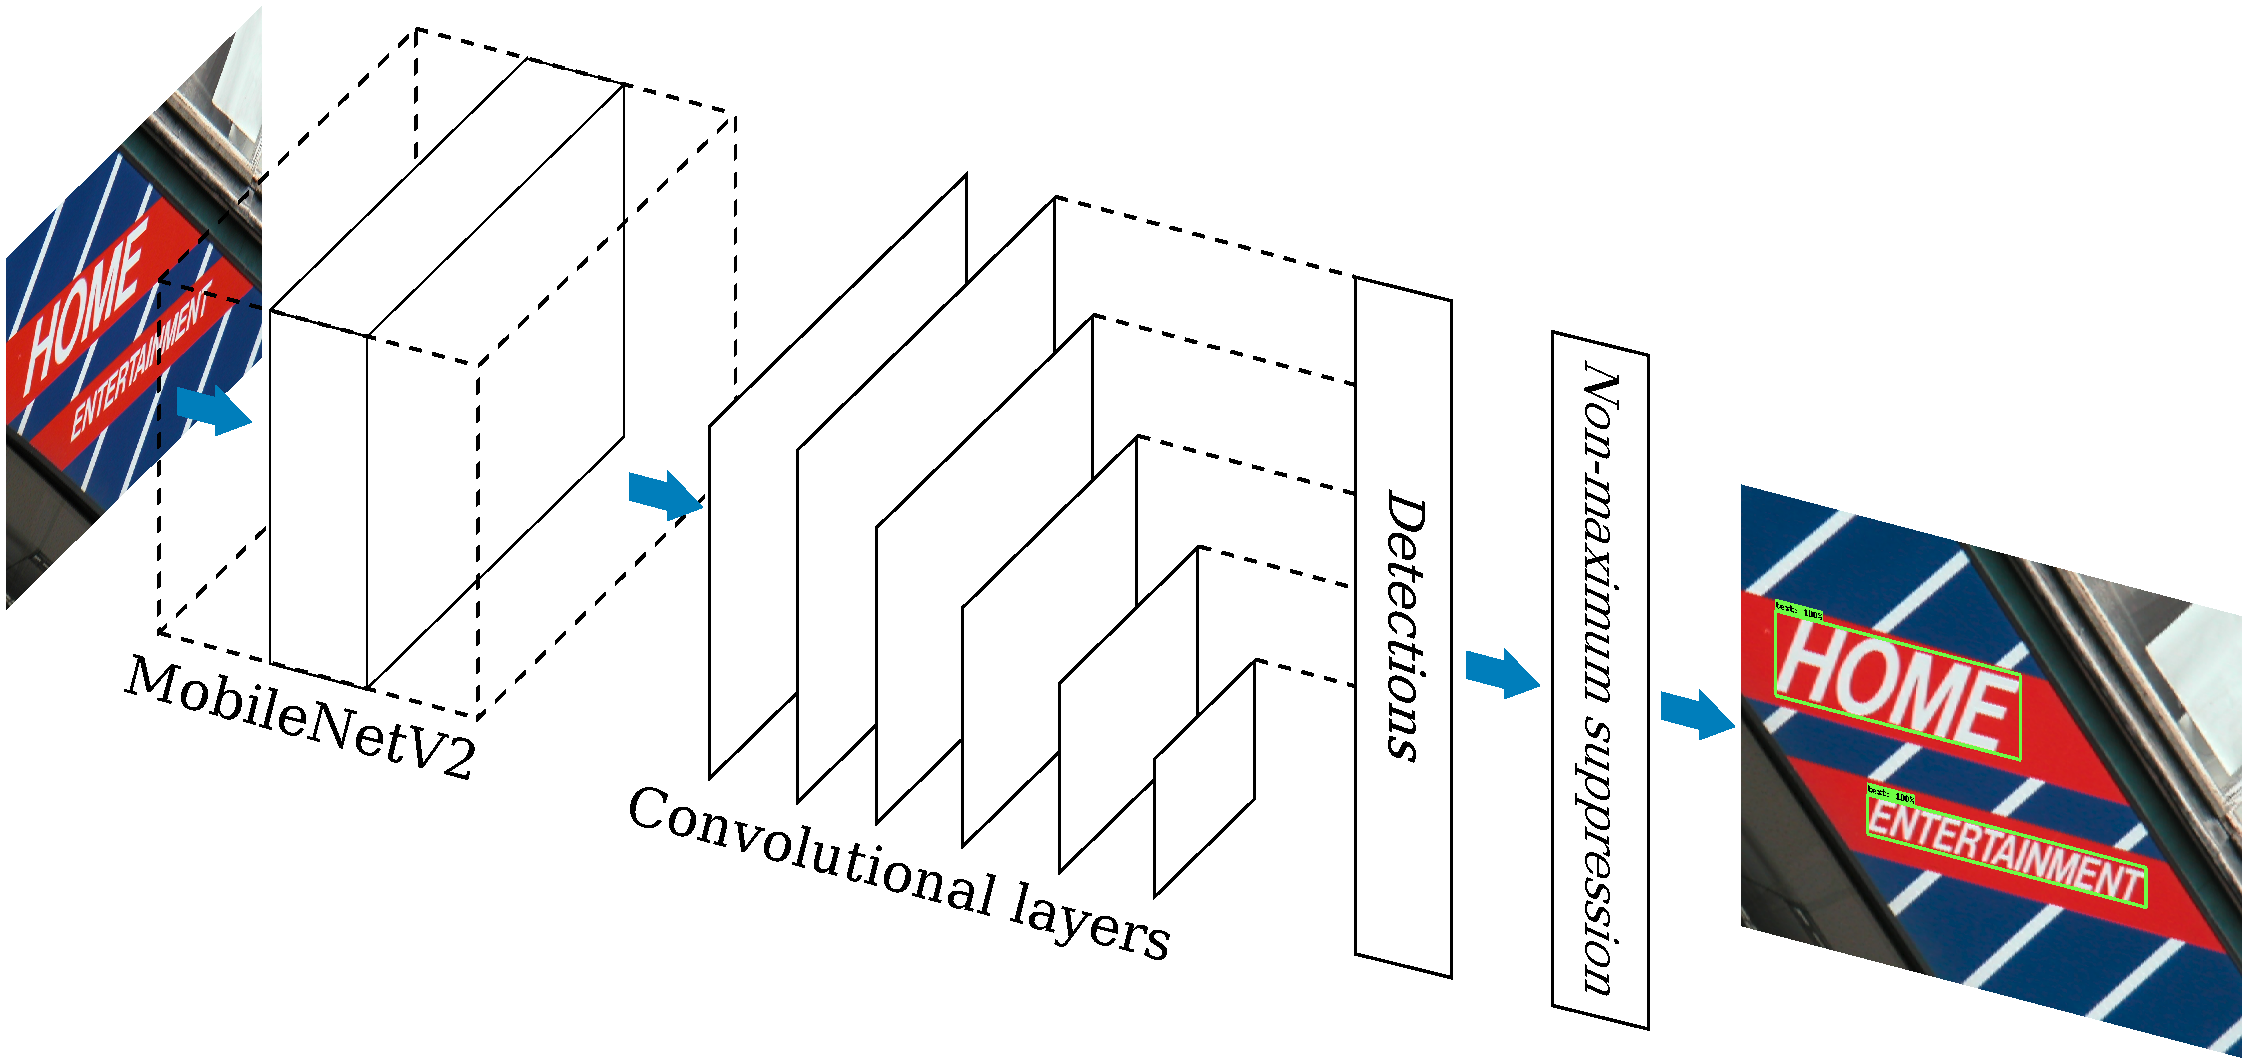
\includegraphics[width=\columnwidth]{ICIP_frankenstein/figs/proposed-method-overview.pdf}
%	\caption{Overview of the proposed method for text localization.}
%	\label{fig:architecture}
%\end{figure}
%\todo[inline]{Move this figure to the "Proposed Method" Section}

% %
% \begin{figure}[!t]
% 	\centering
% 	
\includegraphics[height=0.066\textheight]{figs/examples/img_22.jpg}
% %	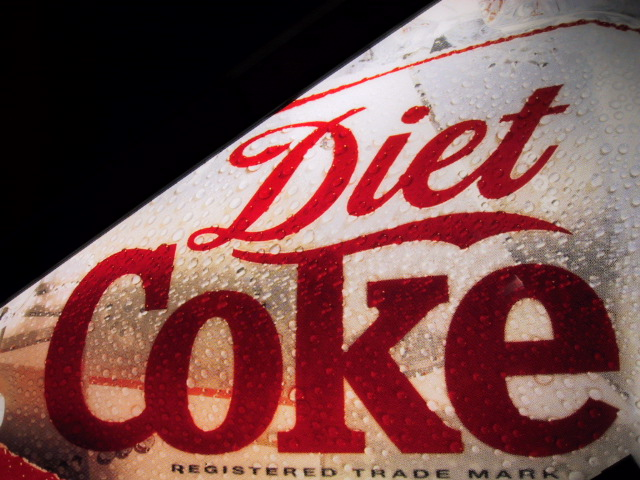
\includegraphics[height=0.08\textheight]{figs/examples/img_42.jpg}
% %	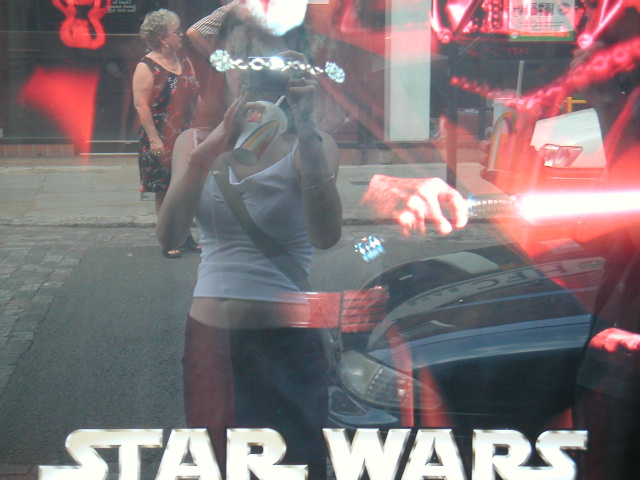
\includegraphics[height=0.08\textheight]{figs/examples/img_108.jpg}
% 	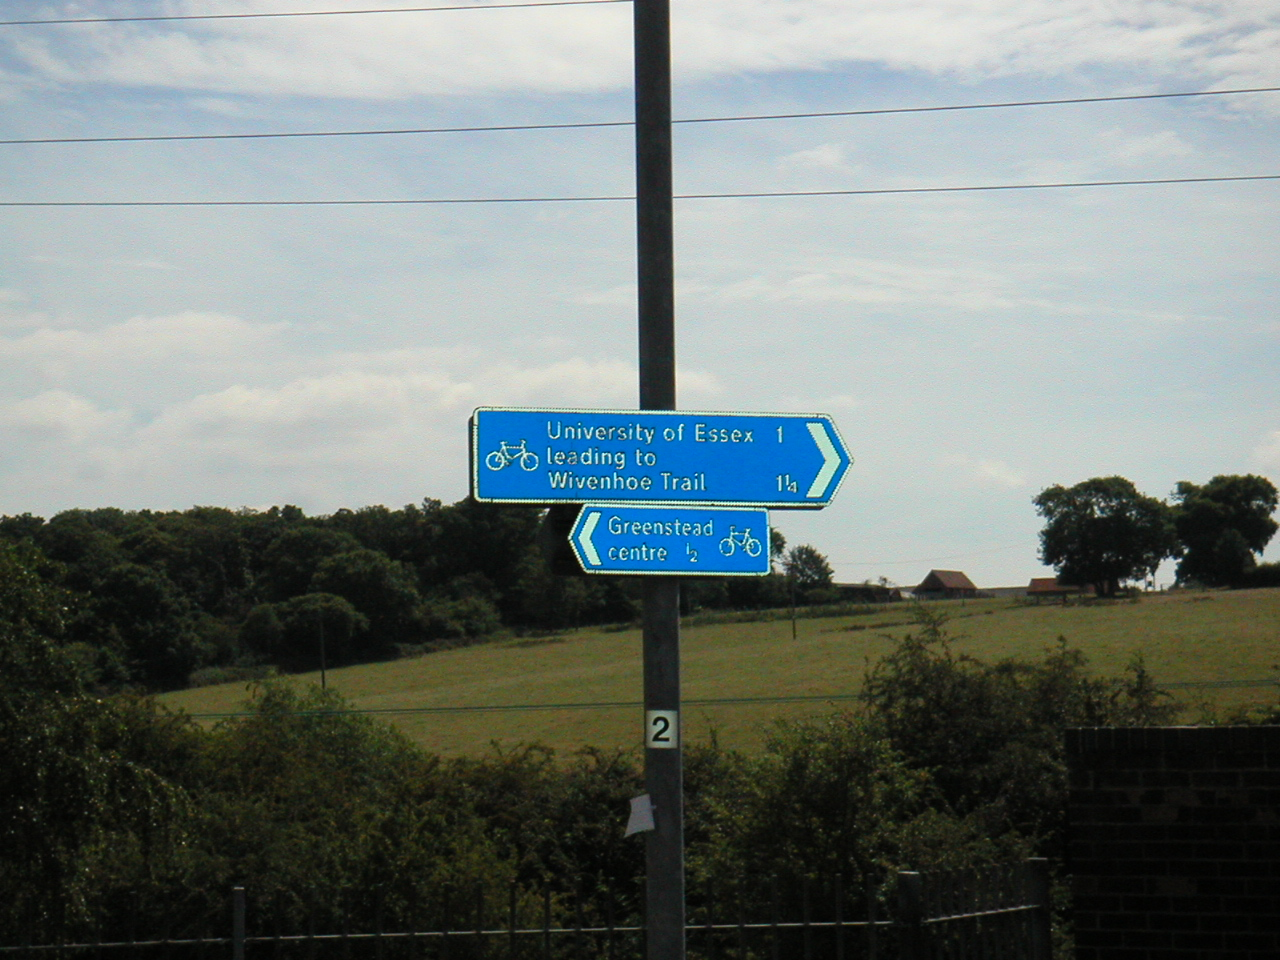
\includegraphics[height=0.066\textheight]{figs/examples/img_126.jpg}
% 	
\includegraphics[height=0.066\textheight]{figs/examples/img_134.jpg}
% 	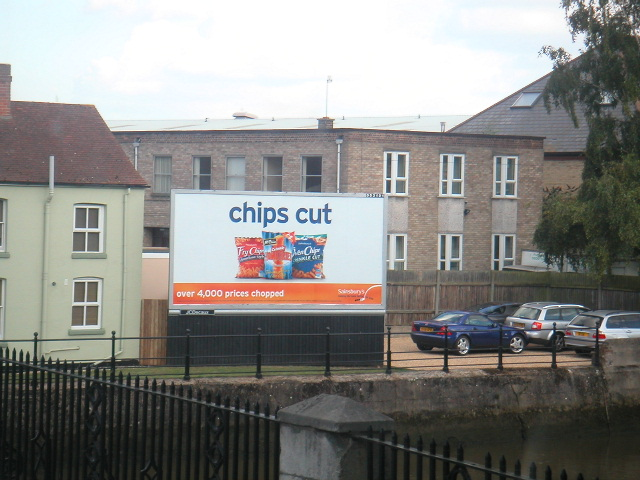
\includegraphics[height=0.066\textheight]{figs/examples/img_175.jpg}
% 	\caption{Example of challenge scene texts.}
% 	\label{fig:dataset-examples}
% \end{figure}
% %

Among the several approaches for localizing text in images, deep-learning-based techniques are the most promising strategies to reach high detection accuracy. \etal{He}~\cite{He2016TIP}, for example, presented a novel technique for scene text detection by proposing a Convolutional Neural Network (CNN) architecture that focuses on extracting text-related regions and specific characteristics of a text. The authors introduced a deep multi-task learning mechanism to train the Text-CNN efficiently, in which each level of the supervised information (text/non-text label, character label, and character mask) is formulated as a learning task. Besides, the authors proposed a pre-processing method, which extends the widely used Maximally Stable Extremal Regions (MSERs)~\cite{Matas2004IVC} by enhancing the local contrast between text and background regions. %The authors reported significant improvements in terms of recall and precision rates, in comparison with methods designed with traditional machine learning techniques for characterizing and learning high level information~\cite{Minetto2014CVIU}. 
Although the proposed CNN presented a reasonable efficiency in detecting candidate regions, with a processing time of about $0.5$ seconds per image, the pre-processing step requires about $4.1$ seconds per image, which may prevent a real-time detection. 

Another venue that may render outstanding results in terms of effectiveness consists of combining different deep learning architectures to benefit from complementary information to make a better decision. In this vein, \etal{Zhang}~\cite{Zhang2016CVPR} introduced an approach based on two Fully Convolutional Network (FCN) architectures for predicting a salient map of text regions in a holistic manner (named as \textit{Text-Block FCN}), and also for predicting the centroid of each character. The main idea of this approach consists of detecting text line blocks, which are more stable in comparison with character regions. Similarly, \etal{Tang} also proposed an ensemble of three modified VGG-16 networks~\cite{Tang2017TIP}: the first extracts candidate text regions (CTR); % of the scene image;  
the second network refines the coarse CTR detected by the first model, segmenting them into text; and finally, the refined CTR are served to a classification network to filter non-text regions and obtain the final text regions. The CTR extractor network is a modified VGG-16 that, in the training process, receives the edges of the text as supervisory information in the first blocks of convolutional layers and the segmented text regions in the last blocks. %Undoubtedly, 
Both strategies present several issues in terms of computational efficiency that could make their use unfeasible in restrictive computing scenarios.% (e.g., mobile devices).

Towards having a truthfully single-stage text detection, \etal{Liao}~\cite{Liao2018TIP} proposed an end-to-end solution named TextBoxes++, which handles arbitrary orientation of word bounding boxes, whose architecture inherits from the VGG-16 architecture. Similarly to TextBoxes++, \etal{Zhu} proposed a deep learning approach~\cite{Zhu2018TITS} also based on the VGG-16 architecture, but for detecting text-based traffic sign. Both techniques presented outstanding detection rates, but they rely on the use of VGG-16 architecture, which could be considered inadequate for restrictive computing scenarios due to its model size with about $138$ millions of parameters~\cite{Howard2017CoRR}, and floating-point operations per second (FLOPS) that reach about $15.3$ billion~\cite{HeCVPR2016}. In contrast, lighter CNN architectures, such as MobileNet~\cite{Howard2017CoRR}, present a very competitive alternative for this scenario, with a model size of $4.2$ millions of parameters and the FLOPS of $569$ million, for instance.

In light of these remarks, we propose a novel method for text localization considering efficiency and effectiveness trade-offs. Our approach, named MobText, combines two light architectures that were originally proposed for object detection -- MobileNetV2~\cite{Sandler2018CVPR} and SSD~\cite{Liu2016ECCV} -- and adapts them to our problem. The main contributions of this work are: 

\begin{itemize}
    \item (i) the proposal of an effective method for text localization task in scene images, which presented better or competitive results when compared with state-of-the-art methods at a low computational cost in terms of model size and processing time; 
    \item (ii) a comparative study, in the context of text localization, comprising widely used CNN architectures recently proposed for object detection;
    \item (iii) state-of-the-art results on the ICDAR'11 dataset, with F-Measure of $96.09\%$, and competitive results on ICDAR'13 with F-Measure of $73.58\%$; and
    \item (iv) proposal of an evaluation tool to support the assessment of text localization and recognition methods. %\todo[inline]{Provide contribution and adapt introduction to tool description}
\end{itemize}
%; and (iii) a study the most promising deep learning techniques for text recognition task?.

In summary, we addressed the following research questions:
\begin{itemize}
    \item Would a general-purpose object detection network, trained for the text detection task, achieve competitive results, in comparison with state-of-the-art methods?
   % \todo[inline]{Suggestion: Can an object detection network, trained for the text detection task, achieve competitive results, in comparison with state-of-the-art methods?}
    \item Would a mobile-oriented CNN architecture maintain a competitive performance on text detection while being light enough to be executed on devices with restricted computing power and built-in memory capacity?
    %\todo[inline]{Suggestion: Can a mobile-oriented CNN architecture maintain a competitive performance on text detection while being light enough to be executed on devices with restricted computing power and built-in memory capacity?}
    
    \item How to devise a generic evaluation tool to support the assessment of text localization and recognition methods?
\end{itemize}


%\etal{Gupta}~\cite{Gupta2016CVPR} proposed a new method for generating synthetic data for the text spotting problem, by blending synthetic text in natural images in order to have a scene text-like dataset, as illustrated in Figure~\ref{fig:Gupta2016CVPR-pipeline.png}. The authors also proposed a new FCN architecture for text/non-text detection. The SynthText dataset consists of synthetic text-scene images produced by a generation engine that localize the best location in a given image (e.g., contiguous regions) by using segmentation and geometry estimation algorithms and render a synthetic text in the found regions taking into account the local color and texture information to produce realistic scene-text images. The FCN network proposed by the authors based on \etal{Long}~\cite{Long2015CVPR} and \etal{Redmon}~\cite{Redmon2016CVPR} works. According to the authors, the improvements made in the YOLO architecture~\cite{Long2015CVPR} was crucial to achieve good results, in terms of accuracy, at a lower computation cost. The effectiveness of the proposed method was confirmed on ICDAR'11 and ICDAR'13 datasets, whose results were superior to works proposed in~\cite{Wang2012ICPR,Jaderberg2016IJCV,Neumann2012CVPR,Zhang2015CVPR}.

The remaining of this dissertation is organized as follows. Chapter~\ref{chap:related-work} introduces basic concepts related to the text detection problem, along with a brief background of technologies and techniques employed in this dissertation. Chapter~\ref{chap:proposed-method} presents MobText, the proposed method for text detection, besides the datasets, evaluation metrics, and protocols used to validate our approach, in comparison with baselines and their usage in real-world usage scenarios involving the use of mobile devices. This chapter also presents and discusses experimental results. %A description of the experiments made on a mobile, restrictive computing environment is provided in Chapter~\ref{chap:mobile-results}.
Chapter~\ref{chap:tool} describes the developed tool to support the evaluation of text localization and recognition methods.
Chapter~\ref{chap:conclusions} provides our conclusions over the results of our research and points out possible future work. 



